\documentclass[landscape,twocolumn]{article}
\title{Atreus Keyboard Assembly}
\date{ }
\usepackage{pdflscape}
\usepackage{graphicx}
\usepackage[landscape,twocolumn]{geometry}
\usepackage{wrapfig}
\newgeometry{margin=2cm}
\begin{document}
\setlength{\columnsep}{1.4cm}
\setlength{\parindent}{0cm}
\maketitle
\section{Prerequisites}

Before starting, make sure your kit has all its parts:

\begin{itemize}
\item Case: top plate, switch plate, spacer pieces, bottom plate
\item Sandpaper: 100-220 grit and 1000-2000 grit waterproof
\item Key switches: 42 tactile or clicky, 5 red optional
\item Printed circuit board (PCB)
\item A-Star Micro controller\footnote{The controller and diodes will be
  attached to the PCB already in presoldered boards.}
\item Diodes\textsuperscript{1}: 42
\item USB micro cable
\item Key caps: 40 normal, 2 long
\item Screws and nuts: 8 each, 16mm M3 size
\item Rubber feet
\end{itemize}

You'll also need to have these on hand:

\begin{itemize}
\item Can of spray lacquer, shellac, or polyurethane (for wood cases)
\item Newspaper or other material to spray on (for wood cases)
\item Soldering iron and solder (lead-free not recommended)
\item Wire cutters (not needed for presoldered kits)
\item Eye protection for soldering
\end{itemize}

\vspace{1em}

The latest version of this document can always be found
online.\footnote{https://atreus.technomancy.us/assembly.pdf} If you are
hand-wiring a board without a PCB, see the older assembly
guide.\footnote{https://atreus.technomancy.us/assembly-hand-wired.pdf}
The photos in this guide depict Matias switches (with rectangular
switch stems), but you can use Cherry MX switches (with stems shaped
like a +) as well.

\section{Sanding}

Acrylic cases can skip down to the ``Diodes'' step below. Otherwise
start by sanding with your rougher sandpaper. The top side of the top
plate and the bottom side of the bottom plate are the only surfaces
that are exposed to the touch once the keyboard is fully assembled, so
these are the ones you'll need to sand.

\vspace{1em}
\begin{center}
  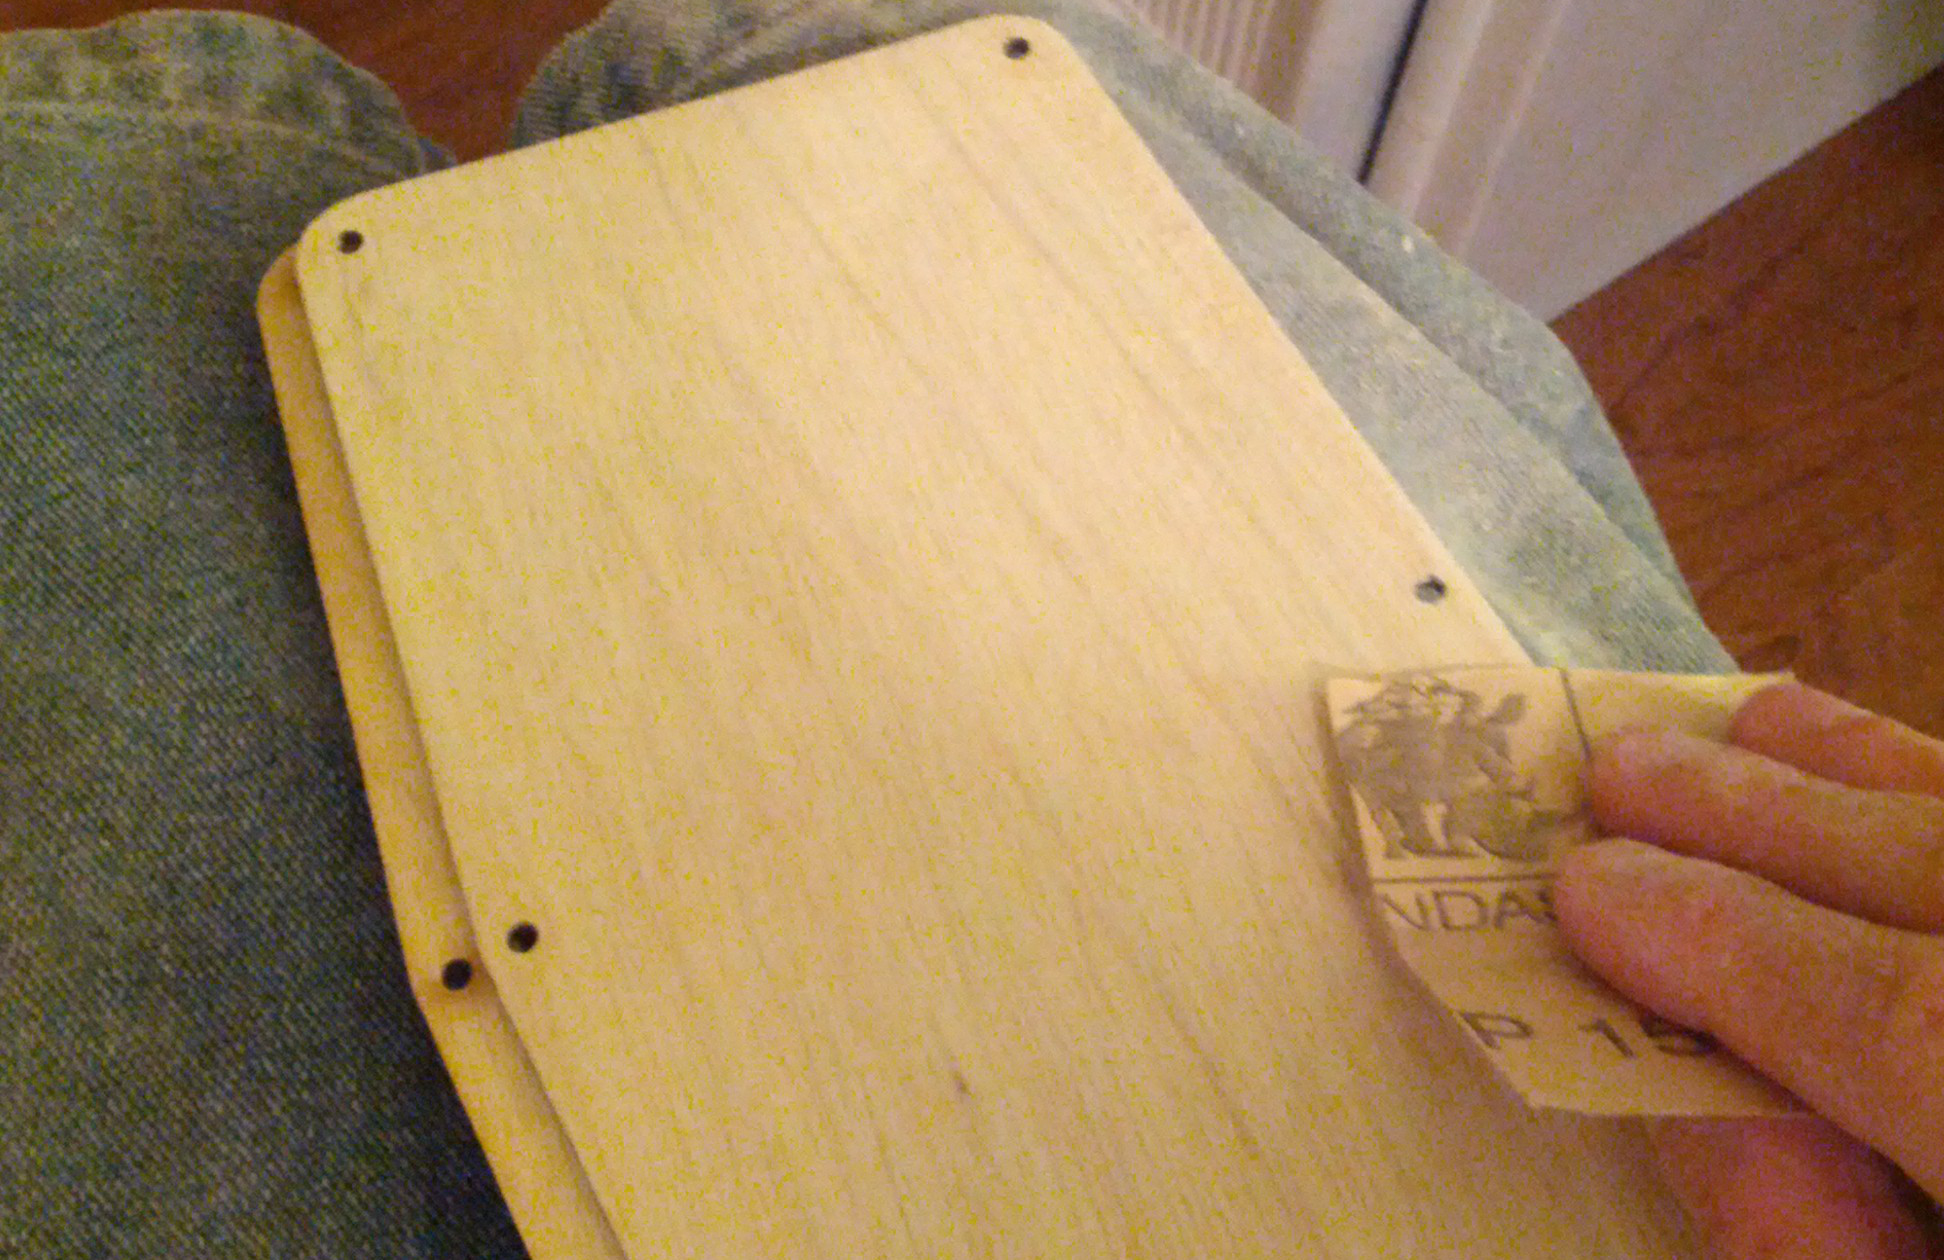
\includegraphics[width=0.7\columnwidth]{sanding.jpg}
\end{center}
\vspace{1em}

You may want to hold two pieces together while sanding for strength or
placing it on a flat surface you don't mind scruffing up; too much
pressure on a single plate could damage it. Be sure to get all the
wood dust off the pieces before you go on. A clean tack cloth or other
fine cloth works well.

\vspace{1em}

Some people don't like the look of the exposed edges charred black
from the laser cutter. You can choose to sand off the charring, or
alternately cover it all with black ink from a sharpie marker for a
more consistent look, or just leave it alone.

\section{Wood Finishing}

Once the case is sanded down all over with coarse sandpaper, find a
good place to spray the lacquer or polyurethane; either outdoors or in
a well-ventilated garage. Lay down the newspaper with the pieces of
the case on top of it. Spray your first coat of lacquer to the face-up
side of each piece. As you spray to and fro, overlapping the path of
the spray slightly will minimize running. The evenness of the spray
matters less on the internal surfaces of the case, so that's a good
place to practice and get the hang of it.

\vspace{1em}

Check the lacquer directions to see how long your particular product
needs to dry; this can vary from half an hour to many hours. Once your
first coat is dry, flip each piece over and spray the other
side. Repeat for a second coat. After the second coat, you can ignore
all surfaces except for the top of the top plate and the bottom of the
bottom plate since only these are exposed to the outside. At this
point you can take in the switch plate and continue the rest of the
keyboard construction in between applying the further coats.

\vspace{1em}

The outer surfaces should have between five to eight coats applied
total. As you get to the later coats, the end result will be smoother
if you can keep them thinner. After your second-to-last coat dries,
take your fine sandpaper and soak it in water, then sand over the top
and bottom surfaces lightly. Add a final coat and buff it with a fine
cloth. If you make any mistakes or are unhappy with the smoothness of
the finish, let it dry and add another layer until you are satisfied.

\section{Diodes}

If you've got a presoldered board, you can skip ahead to the
``Switches'' section.

\vspace {1em}

If you've never soldered before, there are plenty of good
introductions online.\footnote{This one from Adafruit is great:
  https://learn.adafruit.com/adafruit-guide-excellent-soldering/tools}
Coat the tip of the hot iron thinly with some solder before you
start. The key is to use the iron to heat both the hole and the lead
sticking through it for a second or two, then bring in a dab of the
solder. The solder should melt immediately if the joint is hot enough.

\vspace{1em}

Take five diodes at a time and bend them into a U shape. Place them
into the diode holes next to each switch slot on the unlabeled side of
the board. Each diode has a black band on it; the band should be
pointing in the direction of the arrow on the printed side of
the board. Once all five are in, pinch the legs of the diodes together
to keep them from falling out, then flip the board over and solder
them in place. Make sure they don't protrude up more than necessary.

\vspace{1em}
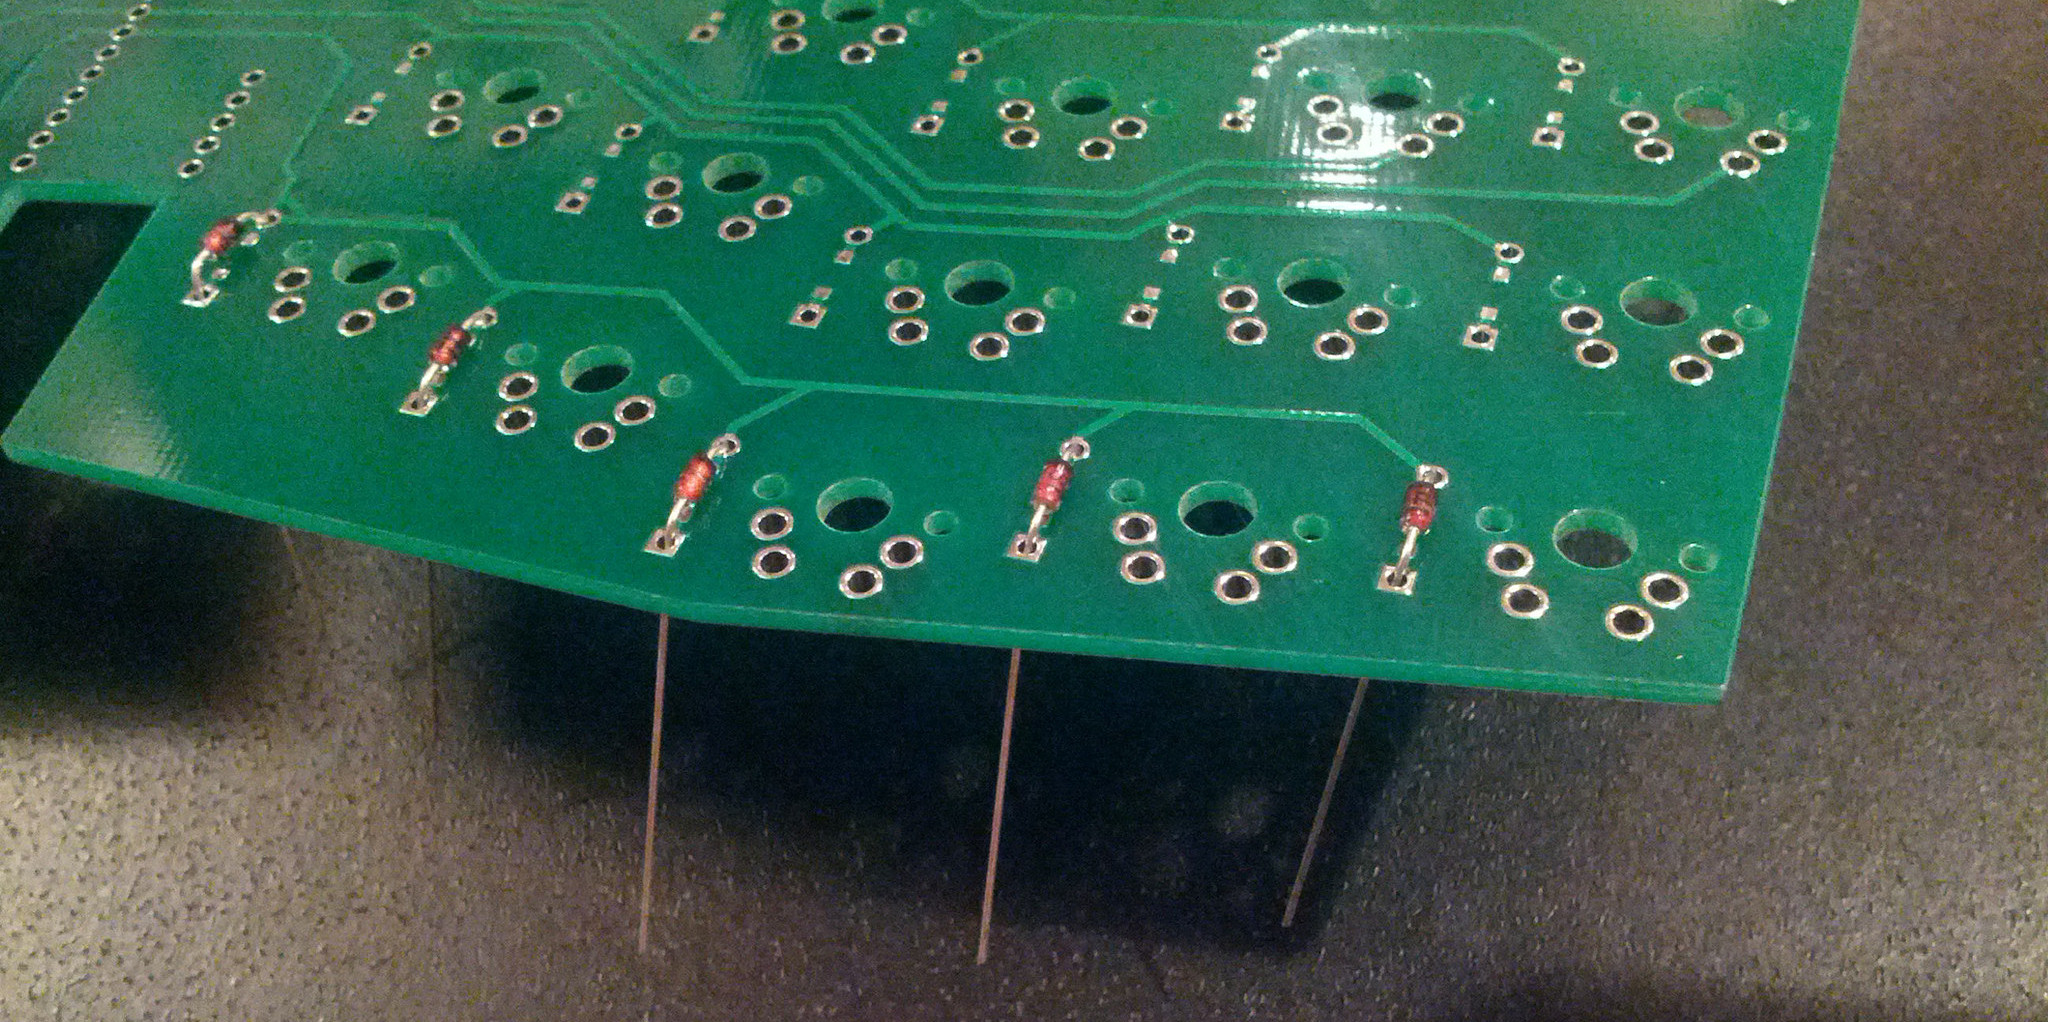
\includegraphics[width=\columnwidth]{diodes.jpg}
\vspace{1em}

Once each set of diodes is soldered, trim the diode legs with wire
cutters. Pinch the diode leg as you trim it to keep it from flying
across the room or into an eye. \textbf{Keep the diode legs}; they will be
needed in the next step. Repeat until each diode position is
filled. Note that each row on the bottom needs six diodes instead of five.

\section{Controller}

Once the diodes are in place, you can begin attaching the controller.
If the controller came in a pink bag with its own header pins, you may
be tempted to use them to connect the controller to the circuit
board. Don't do this--they are too big and will prevent the case from
closing when you're done. We will be using the diode legs we just
trimmed instead.

\vspace{1em}

First take the PCB with the labeled side down and fill the four corner
holes in the center ``A-STAR'' section with solder. Insert diode legs
into these holes while melting the solder. Then repeat the process for
the other holes on the left, keeping them pointing as straight as
possible. Leave the rest of the right side alone for now.

\vspace{1em}
\begin{center}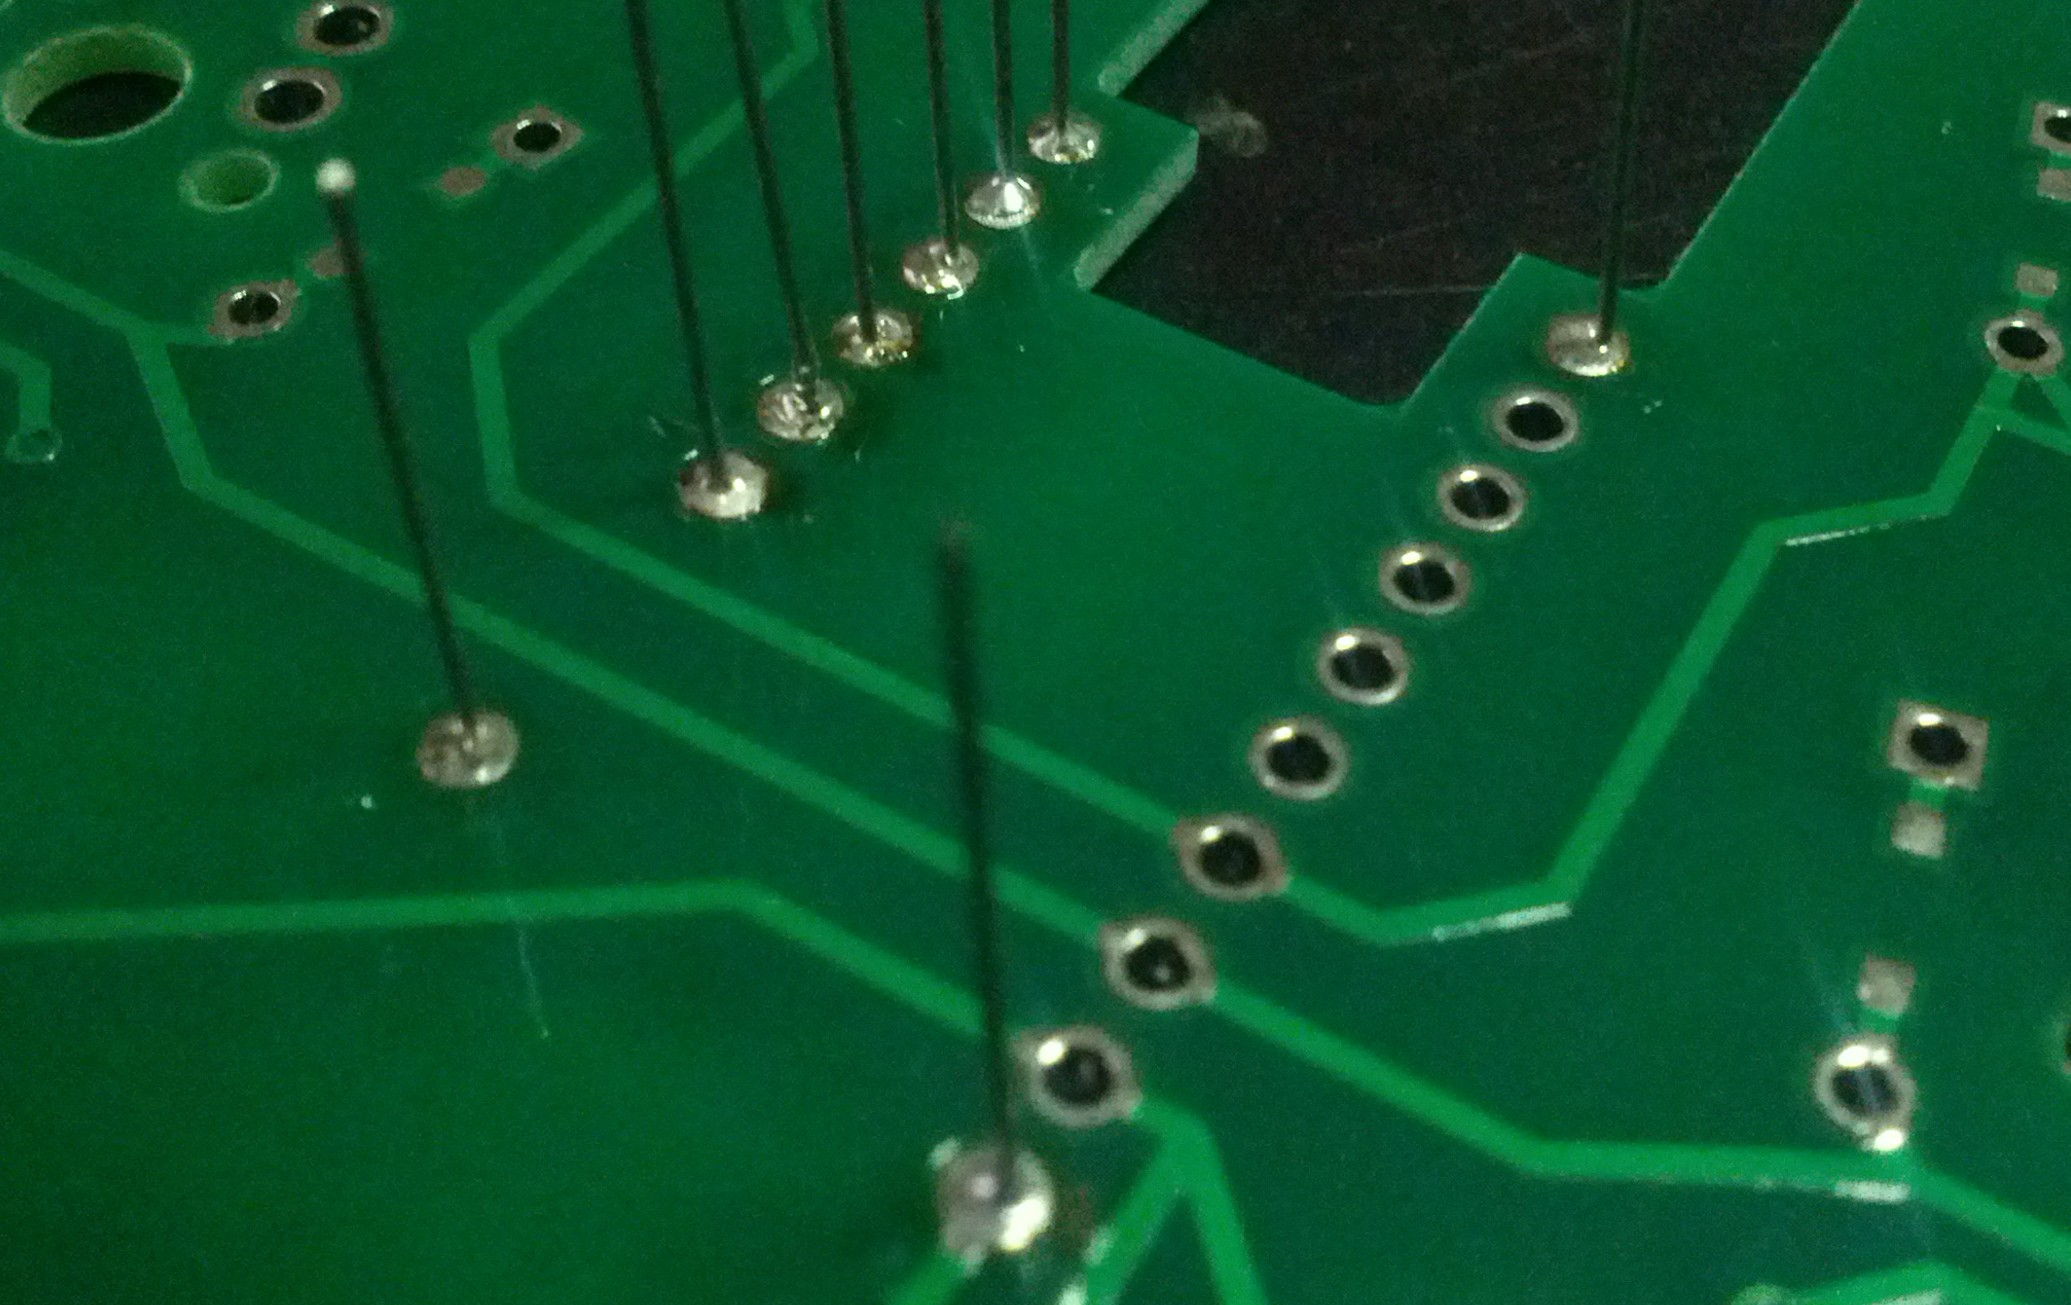
\includegraphics[width=0.8\columnwidth]{many-pins.jpg}\end{center}
\vspace{1em}

Fit the controller over the legs you've attached so far. You can trim
the legs some if it helps get the controller on, but don't cut them to
less than a quarter of the original length. Solder the four corner
pins already connected to the PCB into the corners of the
controller. (The bottom left corner pin of the controller is unused;
the pin above it is used instead.) Try to ensure the controller is as
close to the PCB as possible and not at an angle. Then solder the
other left-side diode legs into the controller as well. Trim them all
with your wire cutters when they are secure.

\vspace{1em}

Eight right-side holes remain. For these, bend four diode legs at a
time into an L shape, and insert them into four of the remaining
holes. Flip the board over and solder the protruding diode legs to the
PCB, then trim them down and flip the board back over. Straighten the
diode legs, then solder and trim them. Repeat for the remaining
right-side holes. From the PCB side, all the holes will be used, but
from the controller side, there will be some unused.

\vspace{1em}
\begin{center}
  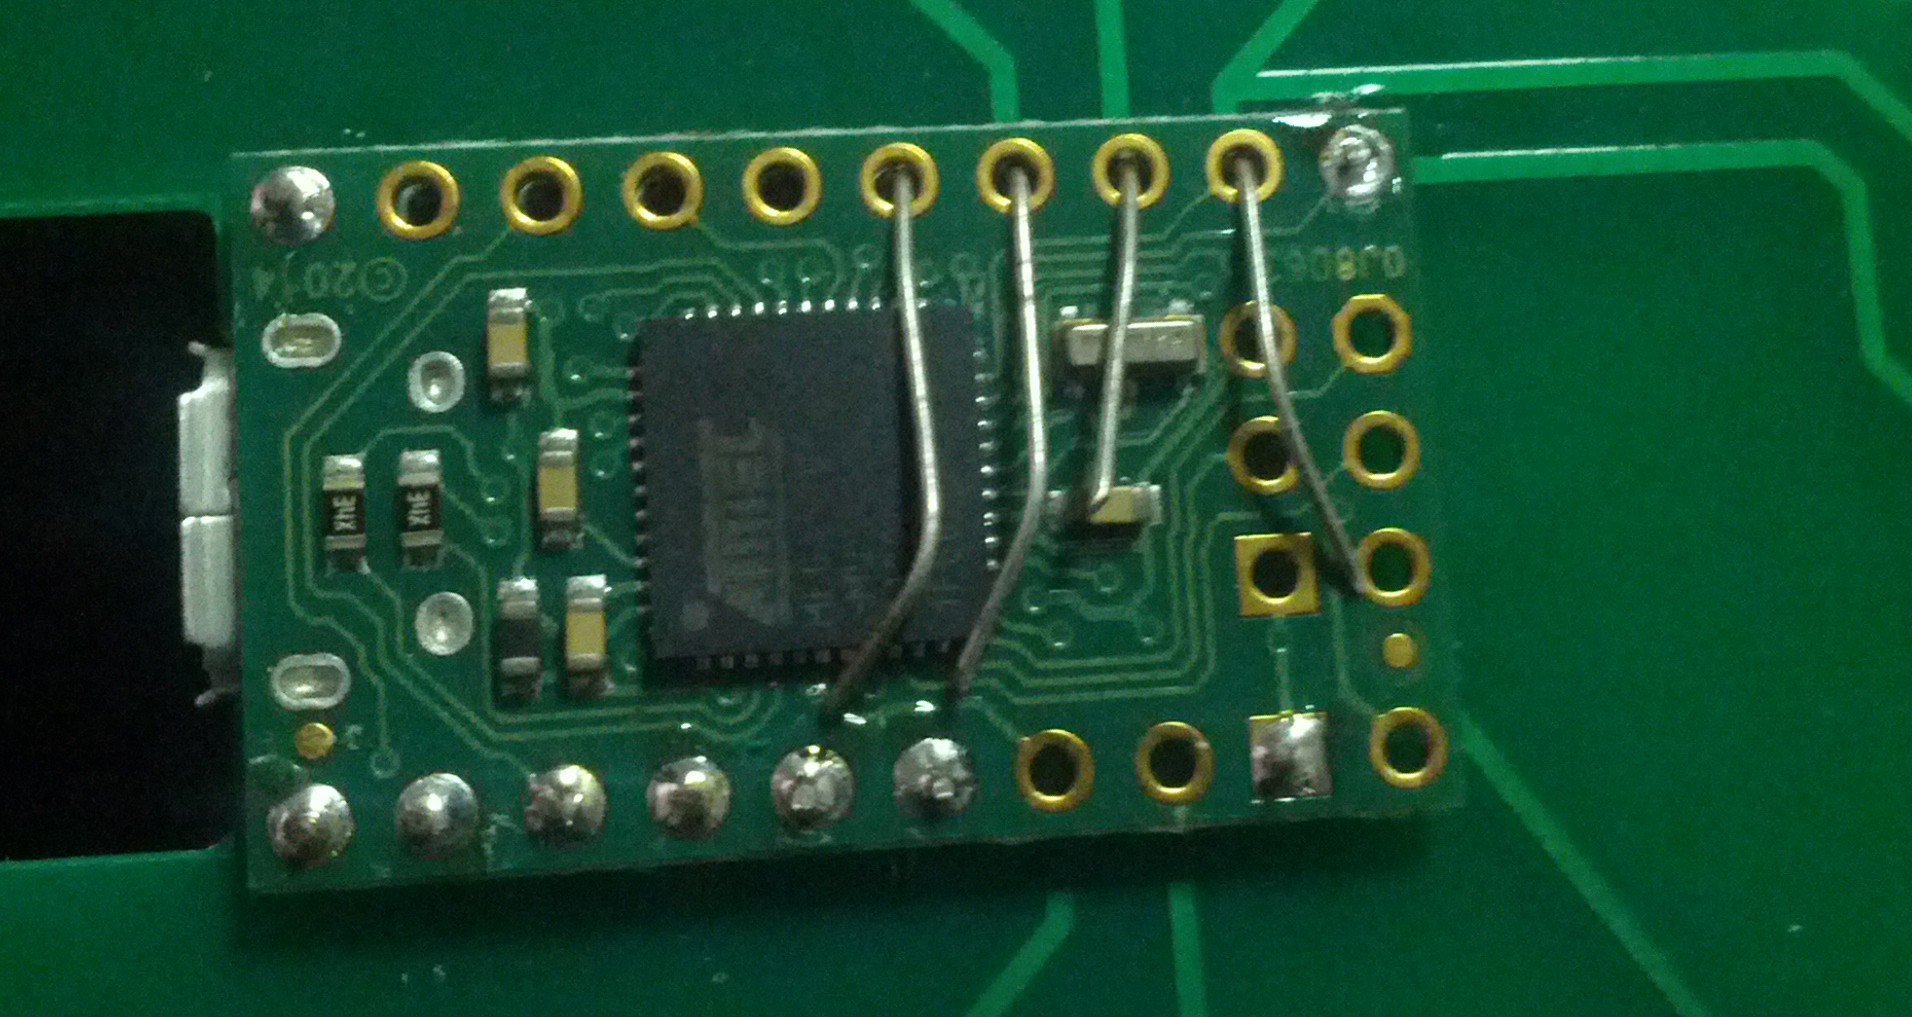
\includegraphics[width=0.8\columnwidth]{bent-legs.jpg}
\end{center}
\vspace{1em}

Before you go on, take the time to double-check the solder joints on
the controller. The solder should fill the hole completely without
spilling over to adjacent holes. Also check that all the diodes are
facing the correct direction with the black band pointing to the
bottom of the board.

\section{Firmware}

Installing the firmware now isn't strictly necessary, but it will
allow you to spot mistakes before the board is finished.

\vspace{1em}

Plug in the USB micro cable into the controller, and plug the other
side into your computer. Get a copy of the
firmware \texttt{.hex} file \footnote{Available at
  https://atreus.technomancy.us/download} and \texttt{avrdude}. The
first time you upload the firmware, you will have to use the hardware
reset to enter the bootloader: take a diode leg or wire and touch one
end to the reset pin and one end to the ground pin. (These are circled
in the photo.)  Touch them together twice in under a second and the
LED underneath will begin pulsing in a smoother pattern from the
original blinking. This indicates it has entered bootloader mode for 8
seconds.

\vspace{1em}

While it's in the bootloader mode, run \texttt{avrdude -p atmega32u4
  -c avr109 -U flash:w:atreus.hex -P /path/to/usb} from the directory
containing the firmware\footnote{See
  https://atreus.technomancy.us/flash for how to determine the USB
  argument and customizing the layout.}. The firmware should be
uploaded, and it will start functioning as a keyboard once switches
are connected. Next time you upload, you can use the reset key instead
of touching the pins together.

\section{Switches}

Next take four switches and place each switch in a corner of the
switch plate. (That's the case layer with all the holes in it.) The
switches should be oriented so that the side with pins is to the
``north'' of the board so they will fit into the holes in the circuit
board. Put the switch plate face-down on the table with the pins
sticking up.

\vspace{1em}

Carefully fit the circuit board over the protruding pins with the
labeled side down. Solder those corners to hold the circuit board and
the switch plate together. The switches should be flush with the
PCB. Take care that the switch pins are straight when you insert them;
pushing in a switch with a pin that's a bit bent will bend it flat and
prevent it from poking through the circuit board.

\vspace{1em}
\begin{center}
  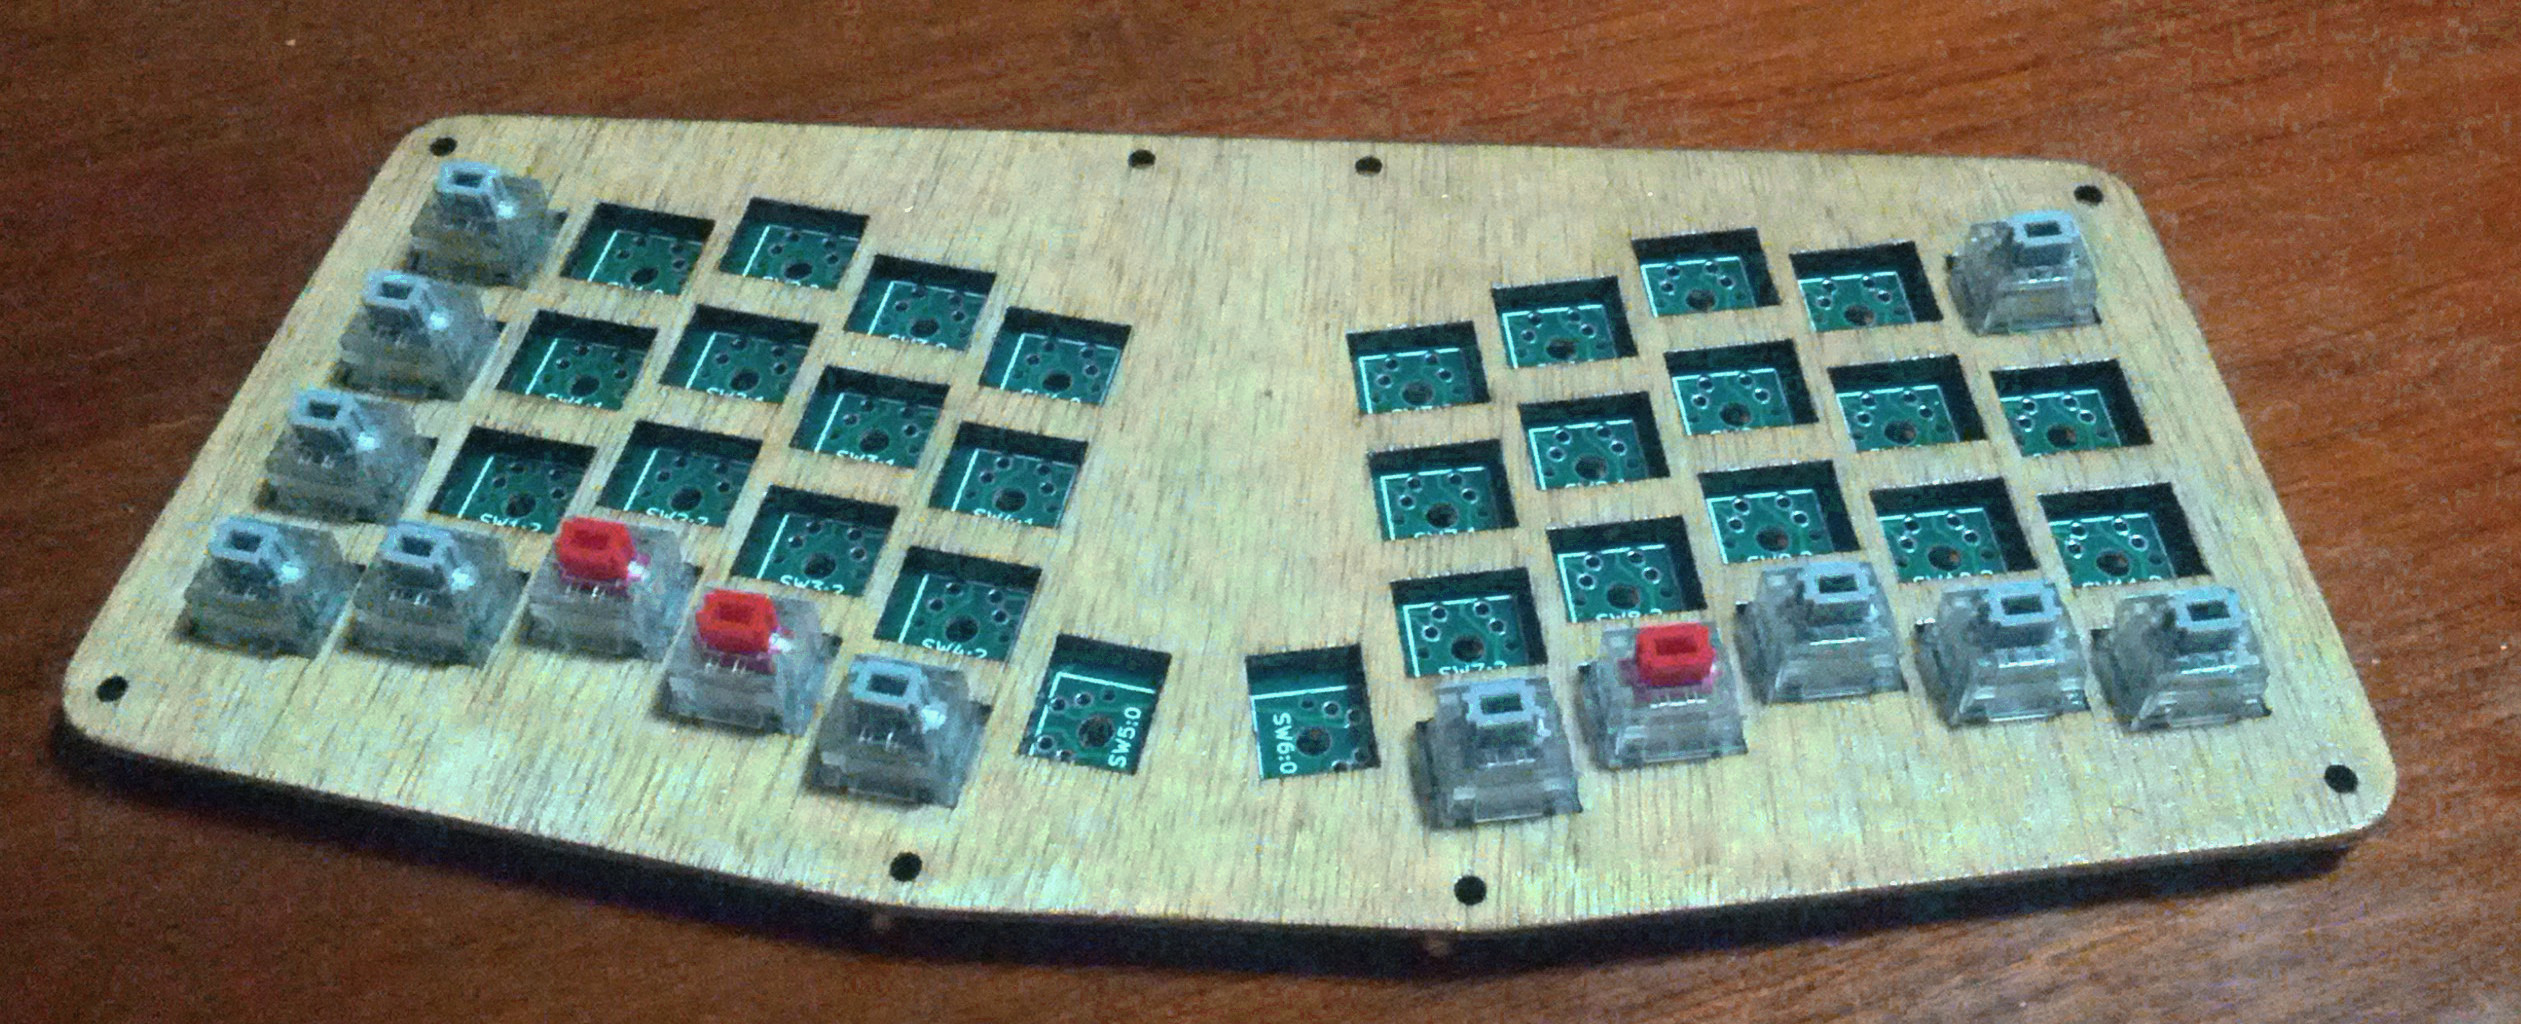
\includegraphics[width=0.9\columnwidth]{some-switches.jpg}
\end{center}
\vspace{1em}

Next fill in the rest of the bottom row (SW1:3 through SW10:3) and the
leftmost column (SW0:1 and SW0:2). If your kit has red linear switches
which do not have any tactile bump, you can choose to use these for
the modifier keys (shift, ctrl, alt, etc) or to leave the modifiers
using the same switches as the rest of the board.\footnote{Since
  modifier keys are held down, they do not benefit from tactility like
  normal keys do, so some people find they prefer linear keys there,
  but this is a matter of personal taste.} The modifiers on the bottom
row are SW2:3, SW3:3, and SW8:3 in the default layout.

\vspace{1em}

Solder the left and right pins of each of the switches you've placed
so far, and then plug it in to a computer to test them to ensure that
each row and column is connected back up to the controller
correctly. Once you've confirmed this, solder the rest of the
switches.

\section{Wrapping Up}

If there's a misbehaving switch, it's often caused by a cold
joint. Reflow the solder on both contacts of the switch and the
diode. If an entire row or column is affected, it's probably the
connection to the controller. You can follow the traces for the rows
back to the middle, but the columns on the back of the board are
obscured when the keyboard is assembled; you can see them in this PCB
diagram\footnote{https://atreus.technomancy.us/pcb}. Re-melting the
controller's solder joint for the affected row or column is usually
enough to get it working. If you still can't
get it working, email me: \texttt{phil@hagelb.org}.

\vspace{1em}

You may want to add strain relief by wrapping the USB cable with
electrical tape at the point just below where it leaves the case. This
will make it so pulling on the cable does not dislodge it from the
controller.

\vspace{1em}

After the switches are all in and tested, place the keycaps. They can
take a fair bit of pressure to go on, so support the underside of the
board while pushing them on. Once the caps are on, they are very
difficult to remove again; don't try to pull them off without
desoldering\footnote{Desoldering a single switch can be done with just
  an iron, but for doing more you may want a pump or wick. See
  https://blog.adafruit.com/2015/11/25/collins-lab-desoldering/} the
switch first.

\vspace{1em}

All that's left is to do is close the case by placing the spacer
pieces and bottom plate on the keyboard while upside down, then
putting some screws in. Flip it over and place the top plate on, then
attach the nuts. If the controller was not attached close enough to
the circuit board, it may be necessary to sand down the USB connector
to reduce its height in order to close the case. If the rubber feet
don't stay on with the provided adhesive, white glue may be needed to
secure them. If you have some wood finishing oil or beeswax, you can
apply it with your fingers after the feet go on for a shinier surface.

\vspace{1em}

Congratulations! Enjoy your new keyboard. It will take a
considerable adjustment period to get used to it, but it should result
in much more comfortable and effective typing. Also remember that
you're encouraged to customize the layout to make it truly your
own. Happy typing!

\end{document}
